\section{Evaluation}

\subsection{Experiment Setup}
For our initial evaluation/experimentation, we use Emulab \cite{2}. Emulab gives us the ability to configure arbitrary network topologies and link bandwidths. For a start, each node in our Emulab topology acts as a datacenter and a link connecting two nodes will act as a link in the WAN. We have configured our environment in Emulab by installing Spark and its dependencies.  Below we show the results from running 'word count' on an emulab cluster containing two connected nodes with traffic-shaping on the link. Our dataset is a subset of wikipedia articles, of size 1GB. We split the dataset into two halves and store each half at each node's local storage. Note that Spark requires the data to be stored on either the local filesystem or HDFS. To give our system this illusion while ensuring that data is accessed over the traffic-shaped link , we set up NFS servers at each node and disabled client-side caching. Each emulab node has 2GB RAM, and two Intel Xeon 3.00GHz processors.

\subsection{Overall Job Time}
Figure~\ref{fig:job-time} shows how the job execution time changes as the link bandwidth is varied. This is compared against both workers running on the same node, i.e., without communication over the WAN. Each data point is the mean of three runs. 

\begin{figure}[tb]
\centering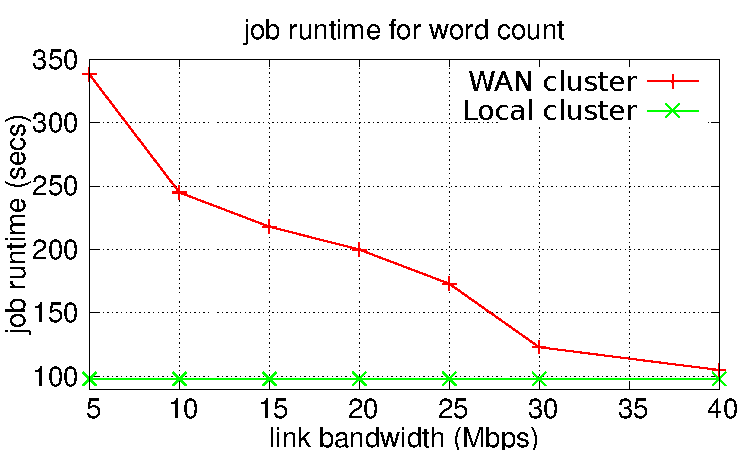
\includegraphics[width=\columnwidth]{figs/job-time.pdf}
\vspace{-1.2em}
\caption{Spark job execution time increases drastically as the WAN link bandwidth goes down.}
\label{fig:job-time}
\vspace{.7em}
\end{figure}


Our next steps are:
\begin{itemize}
\item Use Spark for the data analytics examples described above on an emulated distributed topology and show that as the available network bandwidth is reduced, job times increase.
\item Instrument Spark code to measure the bottleneck computations.
\item Implement the operators needed for our examples.
\end{itemize}

For a specific query, we envision our ‘money-graphs’ to be like this:

\begin{figure}[ht]
	\centering
	\begin{minipage}[b]{0.45\linewidth}
		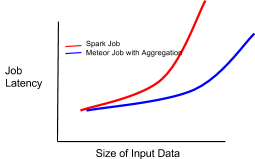
\includegraphics[width=2.3in]{figs/fig_1.png}
		\caption{Latency}
		\label{fig:minipage1}
	\end{minipage}
	\quad
	\begin{minipage}[b]{0.45\linewidth}
		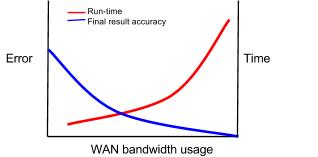
\includegraphics[width=2.6in]{figs/fig_2.png}
		\caption{Error}
		\label{fig:minipage2}
	\end{minipage}
\end{figure}

Here we increase the size of the input data on the x-axis. A Spark job with no topological awareness starts taking longer and longer since the WAN link gets saturated. On the other hand, the corresponding Meteor job takes a lot less time since it uses aggregation to reduce the data needed to be sent over the WAN link. We plan to explore how modulating the bandwidth usage over WAN affects run-time as well as final result accuracy. We expect those result to be highly dependent on the application we are targeting.